\documentclass{midl} % Include author names
%\documentclass[anon]{midl} % Anonymized submission
\usepackage[british]{babel} % decent hyphenation, avoiding e.g. anal-ysis
\usepackage[iso]{isodate}
\usepackage{sansmath}
\usepackage{booktabs}
\usepackage{graphicx}
\usepackage{graphviz}
\usepackage{makecell}
\usepackage{minted}
\usepackage{multicol}
\usepackage{siunitx}
\usepackage{subcaption}
\usepackage[section]{placeins}

% Needs to be loaded after hyperref
\usepackage{cleveref}

% PythonTeX
\usepackage[autoprint=false, gobble=auto, keeptemps=all, pyfuture=all]{pythontex} % create figures on-line directly from python!
\usepackage{pgf}
%\input{/usr/share/repsep/functions.py}
\input{functions.py}
\begin{pythontexcustomcode}[begin]{py}
pytex.add_dependencies(
	'lib/utils.py',
	'lib/categorical.py',
	'data/JogB.tsv'
	)
\end{pythontexcustomcode}
% Single-session PythonTeX codeblocks
\newcounter{pysessioncounter}
\newcommand{\sessionpy}{%
          \edef\sessionpysession{session\arabic{pysessioncounter}}%
            \stepcounter{pysessioncounter}%
              \expandafter\py\expandafter[\sessionpysession]}

% SIunitx customizations detect-all will use the current font for typesetting
\sisetup{per-mode=symbol, detect-all, range-units = single}
\newcommand\SIci[5]{\SI{#1}{#2}, {#3}CI: \SIrange{#4}{#5}{#2}}

% Fix for matplotlib PGF wonkiness which isn't interpreted correctly by pdflatex
\DeclareUnicodeCharacter{2212}{-}

% The following packages will be automatically loaded:
% jmlr, amsmath, amssymb, natbib, graphicx, url, algorithm2e
% ifoddpage, relsize and probably more
% make sure they are installed with your latex distribution

\usepackage{mwe} % to get dummy images

% Header for extended abstracts
\jmlrproceedings{MIDL}{Medical Imaging with Deep Learning}
\jmlrpages{}
\jmlryear{2021}

% to be uncommented for submissions under review
\jmlrworkshop{Short Paper -- MIDL 2021 submission}
\jmlrvolume{-- Under Review}
\editors{Under Review for MIDL 2021}

\title[Multimodal Generative Learning on the MIMIC-CXR Database]{Multimodal Generative Learning on the MIMIC-CXR Database}


% More complicate cases, e.g. with dual affiliations and joint authorship
\midlauthor{\Name{Hendrik Klug\nametag{$^{1}$}} \Email{klugh@ethz.ch}\\
\addr $^{1}$ Institute for Electrical Engineering, ETH Zürich \\
\Name{Thomas M. Sutter\midlotherjointauthor\nametag{$^{2}$}} \Email{thomas.sutter@inf.ethz.ch}\\
\addr $^{2}$ Department of Computer Science, ETH Zürich \AND
\Name{Julia E. Vogt\nametag{$^{2}$}} \Email{julia.vogt@inf.ethz.ch}\\
}

\begin{document}

\maketitle
\begin{abstract}
    Machine Learning (ML) has become more and more popular in the medical domain over the past years.
    While supervised machine learning has received the most attention, unsupervised learning has great potential since there is more data available for the training of the models.
    Especially when leveraging the multi-modal nature of most clinical data, self-supervised learning can provide results comparable to supervised methods.
    Multi-modal unsupervised methods have been tested extensively on toy-datasets like MNIST \cite{lecun-mnisthandwrittendigit-2010, thomas_gener-ELBO, wu2018multimodal} and CelebA \cite{liu2015faceattributes, thomas_gener-ELBO, wu2018multimodal} but to the best of our knowledge have never been applied to medical data, for direct applications such as disease classification and image generation.
    In this article, we apply a method for self-supervised training proposed in \cite{thomas_gener-ELBO} to medical data from the MIMIC-CXR Database \cite{johnson2019mimic} and show that these methods provide promising results on medical data from the MIMIC-CXR database, while highlighting that the task is extremely challenging and that there is space for substantial improvements.
\end{abstract}


\begin{keywords}
Multimodal Learning, Generative Learning, VAE
\end{keywords}

\section{Introduction}

	Manually creating annotations of sufficient training examples for the training of a deep learning model is often infeasible, since it requires manual expert input.
	In the medical domain especially, human labeled data is expensive to acquire and thus very scarce.
	A generative model, that can learn embeddings of the data without the need for labels, enjoys a much bigger variety of possible training data.
	The Variational Autoencoder (VAE) \cite{doersch2016tutorial} in particular is a popular generative model, which consists of an encoder that maps the input to a learned latent distribution from which the decoder part samples to reconstruct the input.

	Clinical data comes in many modalities, such as images, text reports and electronic health records.
	A generative model that can leverage all of the modalities could be used for tasks such as generating a text report when given images of a patient, generating an image of another angle from an input image or data classification.
	However, in contrast to toy datasets, the different pathologies that represent the classes in medical data are defined by very subtle features that only human experts can recognise.
	This makes the task of learning a latent representation of the data, while preserving the separability of the classes extremely challenging.
	
	In this work, we apply the generalised multimodal ELBO, proposed in \cite{thomas_gener-ELBO}, to train a self-supervised, generative model on clinical data from the MIMIC-CXR Database \cite{johnson2019mimic} containing chest-X rays and related text reports. 
	We provide a first insight into the difficulties and opportunities that come with medical data.

\section{Methods}
Assuming the data consists of $N$ i.i.d. samples $\{\xseti\}^N_{i=1}$, each of which is a set of M modalities $\mathbb{X}^{(i)} = \{\textbf{x}_j^{(i)}\}^M_{j=1}$, the joint posterior distribution is calculated in two steps.
In a first step, a distribution is calculated for each subset of the powerset $\powerset$ using a Product of Experts (PoE) \cite{wu2018multimodal}.
In a second step these subsets are merged using a Mixture of Experts (MoE) \cite{shi2019variational} into a joint posterior distribution.

The MIMIC-CXR Database \cite{johnson2019mimic} provides a class-label for every sample, corresponding to one or more of 13 pathologies.
For the evaluation of our method, we created a label "Finding", indicating if the sample is labeled with any of the 13 pathologies. 
All images were resized to (128, 128) and every word that occurs at
least 3 times in all the text reports is mapped to an index. 
Using this mapping each sentence is encoded into a sequence of indices. 
All sentences with a word count above 128 are truncated and all sentences consisting of less words are padded with a padding token "$< pad>$" such that all text samples are of length 128.

\section{Results}

    In the following section, we will abbreviate the three modalities present in the data selection with "F" for frontal scan, "L" for lateral scan and "T" for text report.
    
    \textbf{Evaluation of the latent representation.} \tableref{tab:lr_table} shows the evaluation of linear classifiers that were trained and evaluated on the learned latent representation.
    We note that the uni-modal subspaces provide a less good separability between samples that are labeled with a Finding and samples that are not.
    The highest score is achieved by the classifiers evaluated on the subspace spanned by all three modalities.
    This shows that the information of all modalities are successfully merged in the joint posterior distribution.  
    Overall, the text modality provides the best separability.
    
    \begin{table}[htbp]
    \floatconts
      {tab:lr_table}%
      {\caption{\textbf{Classification results of the linear classifiers trained on the learned latent representation using the binary label "Finding".} 
      The mean average precision over the test set is reported for each modality (F: frontal image, L: lateral image, T: text report).
      The random performance lies at 0.395.}}%
      {\begin{tabular}{llrrrrrrr}
                MODEL & LABEL   & F     & L     & T     & L,F   & F,T   & L,T   & L,F,T          \\
                \midrule
                MoPoE & Finding & 0.467 & 0.460 & 0.473 & 0.476 & 0.493 & 0.475 & \textbf{0.494} \\
    
            \end{tabular}}
    \end{table}
    
    
    \textbf{Generation Quality.} \Cref{fig:fig_cond_lattext} and \cref{fig:fig_cond_latPAtext} compare the generation quality of the model, without the F modality as input as well as given the F modality as conditioner.
    Adding the F modality as input for the generation brings a significant improvement to the quality of the generated samples.
    The generated samples from \cref{fig:fig_cond_latPAtext} are less blurry and smaller details are recognizable.

    \begin{figure}[h]
    \centering
  \hfill
  \begin{minipage}[t]{.45\textwidth}
    \begin{center}  
      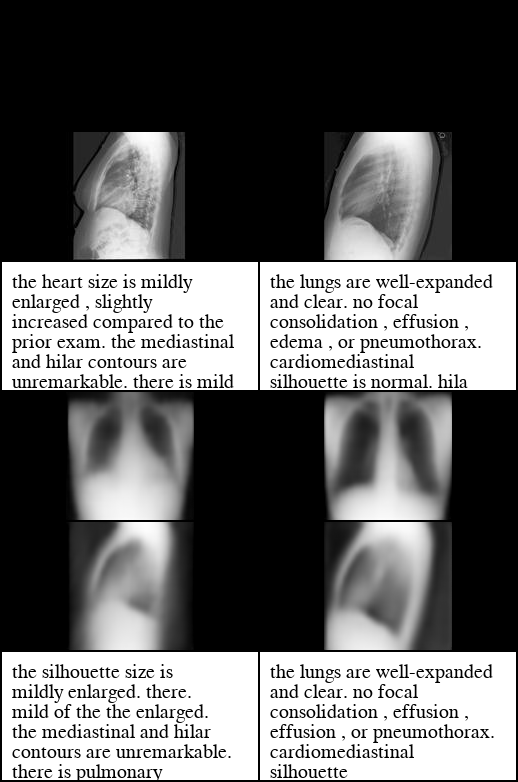
\includegraphics[scale=0.25]{data/cond_gen/Lateral_text_small}
      \caption{\small{\textbf{Conditionally generated samples with L and T modalities as conditioner.} The second and third image rows were given to the model as conditioner. The three last image rows are the generated samples.}}
      \label{fig:fig_cond_lattext}
    \end{center}
  \end{minipage}
  \hfill
  \begin{minipage}[t]{.45\textwidth}
    \begin{center}  
      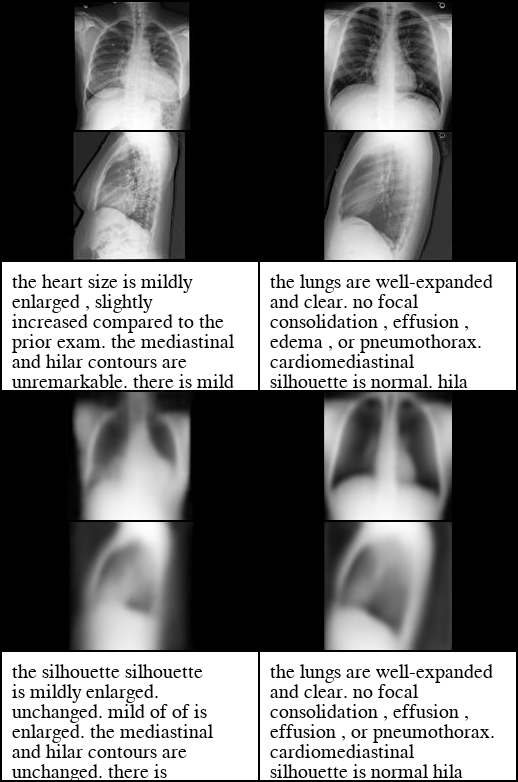
\includegraphics[scale=0.25]{data/cond_gen/Lateral_PA_text_small}
      \caption{\small{\textbf{Conditionally generated samples with F, L and T modalities as conditioner.}}}
      \label{fig:fig_cond_latPAtext}
    \end{center}
  \end{minipage}
  \hfill
    \end{figure}
    
\section{Conclusion}
    In this work, we applied a method for multi-modal generative learning on clinical data and evaluated its performance on direct applications in the medical field.
    
    While our experiments show promising results, they indicate that the task is extremely challenging with significant scope for improvement.
    
    In particular, we showed that features in medical scans that are characteristic of most diseases are often smaller details that get lost in the blurriness of the generated samples.
    However, the latent representation that the MoPoE learns when learning to reproduce the data is still meaningful in the sense that it can be separated into the different classes the data belong to.

    We argue that our method is a successful first step into creating an unsupervised method that will find applications in the medical domain such as classification of diseases, generating text reports from medical data and generating scans from multiple angles.
    However, we believe that the method can be improved with some further fine-tuning, for example in the choice of the abstract mean function for modelling the joint posterior or in the choice of the encoder-decoder architectures.


% Acknowledgments---Will not appear in anonymized version
\midlacknowledgments{We thank a bunch of people.}


\bibliography{bib}


\appendix

\section{Proof of Theorem 1}

This is a boring technical proof of
\begin{equation}\label{eq:example}
\cos^2\theta + \sin^2\theta \equiv 1.
\end{equation}

\section{Proof of Theorem 2}

This is a complete version of a proof sketched in the main text.

\end{document}